\begin{name}
	{\tenchude}
	{\tendethi}
	{LỚP TOÁN THẦY PHÁT}
	{\lq\lq The future starts today, not tomorrow.\rq\rq}
\end{name}

\Opensolutionfile{ans}[ans/De-TB-Yeu-So-3]
\TN
\begin{ex}%[1D2N2-2]
	Trong các dãy số sau, dãy nào là cấp số cộng?
	\choice
	{$1$; $4$; $7$; $10$; $14$}
	{\True $5$; $2$; $-1$; $-4$; $-7$}
	{$-3$; $1$; $5$; $9$; $14$}
	{$\dfrac{1}{2}$; $\dfrac{2}{3}$; $1$; $\dfrac{4}{3}$; $2$}
	\loigiai{
		Dãy số $5$; $2$; $-1$; $-4$; $-7$ là một cấp số cộng vì hiệu của hai số hạng liên tiếp luôn là một hằng số. Thật vậy, ta có
		\[2-5=-1-2=-4-(-1)=-7-(-4)=-3.\]
		Do đó, đây là cấp số cộng có số hạng đầu $u_1=5$ và công sai $d=-3$.
	}
\end{ex}

\begin{ex}%[2D1H3-1]
	Giá trị nhỏ nhất của hàm số $y=\dfrac{x+4}{x-2}$ trên đoạn $[3;4]$ là
	\choice
	{$7$}
	{\True $4$}
	{$-6$}
	{$3$}
	\loigiai{
		Hàm số $f(x)=\dfrac{x+4}{x-2}$ xác định và liên tục trên đoạn $[3;4]$.\\
		Ta có
		$f'(x)=\dfrac{1\cdot (-2)-1\cdot 4}{(x-2)^2}=\dfrac{-6}{(x-2)^2}<0$, $\forall x\in [3;4]$.\\
		Vì $f'(x)<0$ trên đoạn $[3;4]$ nên hàm số $f(x)$ nghịch biến trên đoạn $[3;4]$. \\
		Suy ra giá trị nhỏ nhất của hàm số trên đoạn này đạt được tại $x=4$. \\
		Vậy $\min \limits_{[3;4]}f(x)=f(4)=\dfrac{4+4}{4-2}=4$.
	}
\end{ex}

\begin{ex}%[1D5H2-2]
	Cho mẫu số liệu ghép nhóm về tuổi thọ của một loại máy lọc nước mới như sau
	\begin{longtable}{|l|c|c|c|c|}
		\hline
		Tuổi thọ & $[2;3{,}5)$ & $[3{,}5;5)$ & $[5;6{,}5)$ & $[6{,}5;8)$ \\
		\hline
		Số máy & $8$ & $22$ & $35$ & $15$ \\
		\hline
	\end{longtable}
	Nhóm chứa trung vị của mẫu số liệu là
	\choice
	{$[2;3{,}5)$}
	{$[3{,}5;5)$}
	{\True $[5;6{,}5)$}
	{$[6{,}5;8)$}
	\loigiai{
		Cỡ mẫu là $n=8+22+35+15=80$. \\
		Giả sử dãy số liệu được sắp xếp theo thứ tự tăng dần.\\ Khi đó, trung vị là trung bình cộng của số liệu thứ $40$ và $41$. \\
		Ta có
		\begin{itemize}
			\item Nhóm thứ nhất có $m_1=8$ số liệu.
			\item Tổng số lượng số liệu của hai nhóm đầu là $m_1+m_2=8+22=30$.
			\item Tổng số lượng số liệu của ba nhóm đầu là $m_1+m_2+m_3=30+35=65$.
		\end{itemize}
		Do $30<40<41\le 65$ nên hai giá trị thứ $40$ và $41$ đều thuộc nhóm thứ ba là $[5;6{,}5)$.\\
		Vậy nhóm chứa trung vị của mẫu số liệu là $[5;6{,}5)$.
	}
\end{ex}

\begin{ex}%[2D1N1-2]
	\immini[thm]
	{Cho hàm số $y=f(x)$ xác định trên $\mathbb{R}\setminus\{2\}$ và có bảng biến thiên như hình vẽ bên. Mệnh đề nào dưới đây đúng?
	\choice
	{Hàm số $y=f(x)$ đồng biến trên $\mathbb{R}$}
	{\True Hàm số $y=f(x)$ nghịch biến trên từng khoảng $(-\infty;2)$ và $(2;+\infty)$}
	{Hàm số $y=f(x)$ nghịch biến trên $\mathbb{R}$}
	{Hàm số $y=f(x)$ đồng biến trên từng khoảng $(-\infty;2)$ và $(2;+\infty)$}}
	{
\begin{tikzpicture}
			\tkzTabInit[lgt=1.2,espcl=2.5] 
			{$x$/0.6,$f'(x)$/0.6,$f(x)$/2.5} {$-\infty$,$2$,$+\infty$}
			\tkzTabLine{,-,d,-,}
			\tkzTabVar{+/ $1$,-D+/ $-\infty$ / $+\infty$,-/ $1$}
	\end{tikzpicture}}
	\loigiai{
		Dựa vào bảng biến thiên, ta thấy $f'(x)<0$ với mọi $x\in (-\infty;2)$ và $x\in (2;+\infty)$. \\
		Do đó, hàm số $y=f(x)$ nghịch biến trên từng khoảng $(-\infty;2)$ và $(2;+\infty)$.
	}
\end{ex}

\begin{ex}%[1D6H4-2]
	Nghiệm của phương trình $\log _3x=2$ là
	\choice
	{$x=6$}
	{\True $x=9$}
	{$x=5$}
	{$x=8$}
	\loigiai{
		Điều kiện xác định $x>0$.\\
		Ta có
		\[\log _3x=2\Leftrightarrow x=3^2\Leftrightarrow x=9.\]
		So với điều kiện, ta thấy $x=9$ thỏa mãn. \\
		Vậy nghiệm của phương trình là $x=9$.
	}
\end{ex}

\begin{ex}%[2D4N1-3]
	Tìm họ nguyên hàm của hàm số $f(x)=\cos 2x$.
	\choice
	{\True $\displaystyle\int f(x)\mathrm{\,d}x=\dfrac{1}{2}\sin 2x+C$}
	{$\displaystyle\int f(x)\mathrm{\,d}x=2\sin 2x+C$}
	{$\displaystyle\int f(x)\mathrm{\,d}x=-\dfrac{1}{2}\sin 2x+C$}
	{$\displaystyle\int f(x)\mathrm{\,d}x=-2\sin 2x+C$}
	\loigiai{
		Ta có
		\[\displaystyle\int f(x)\mathrm{\,d}x=\displaystyle\int \cos 2x\mathrm{\,d}x=\dfrac{1}{2}\sin 2x+C.\]
	}
\end{ex}

\begin{ex}%[2H5H3-2]
	Trong không gian với hệ tọa độ $Oxyz$, mặt cầu nào có tâm nằm trên mặt phẳng tọa độ $(Oxy)$?
	\choice
	{$(S_3)\colon x^2+y^2+z^2+2x-6z-2=0$}
	{\True $(S_1)\colon x^2+y^2+z^2+2x-4y-2=0$}
	{$(S_4)\colon x^2+y^2+z^2+2x-4y+6z-2=0$}
	{$(S_2)\colon x^2+y^2+z^2-4y+6z-2=0$}
	\loigiai{
		Mặt phẳng tọa độ $(Oxy)$ có phương trình là $z=0$.\\ Do đó, một điểm nằm trên mặt phẳng $(Oxy)$ khi và chỉ khi cao độ của nó bằng $0$.\\
		Xét mặt cầu $(S_1)\colon x^2+y^2+z^2+2x-4y-2=0$, phương trình có thể viết lại dưới dạng
		\[(x+1)^2+(y-2)^2+z^2=7.\]
		Tâm của mặt cầu $(S_1)$ là điểm $I(-1;2;0)$. \\
		Vì cao độ $z_I=0$ nên tâm $I$ nằm trên mặt phẳng $(Oxy)$.
	}
\end{ex}

\begin{ex}%[1D6N4-2]
	Biết $y=\log _2x$. Khi đó
	\choice
	{$x=2y$}
	{\True $x=2^y$}
	{$y=2^x$}
	{$x=y^2$}
	\loigiai{
		Theo định nghĩa của logarit: với $a>0$, $a\neq1$ và $x>0$, ta có $\log _ax=y\Leftrightarrow x=a^y$.\\
		Áp dụng định nghĩa trên với cơ số $a=2$, ta suy ra
		\[y=\log _2x\Leftrightarrow x=2^y.\]
	}
\end{ex}

\begin{ex}%[2D4N2-2]
	Nếu $\displaystyle\int \limits_1^2f(x)\mathrm{\,d}x=-2$ và $\displaystyle\int \limits_2^3f(x)\mathrm{\,d}x=1$ thì $\displaystyle\int \limits_1^3f(x)\mathrm{\,d}x$ bằng
	\choice
	{$-3$}
	{$3$}
	{$1$}
	{\True $-1$}
	\loigiai{
		Ta có
		\[\displaystyle\int \limits_1^3f(x)\mathrm{\,d}x=\displaystyle\int \limits_1^2f(x)\mathrm{\,d}x+\displaystyle\int \limits_2^3f(x)\mathrm{\,d}x=-2+1=-1.\]
	}
\end{ex}

\begin{ex}%[2D6H1-2]
	Cho hai biến cố $A$, $B$ với $\mathrm{P}(A)=0{,}5$; $\mathrm{P}(B)=0{,}8$ và $\mathrm{P}(A\cap B)=0{,}38$. Tính xác suất của $\mathrm{P}(A\mid B)$.
	\choice
	{$0{,}52$}
	{$0{,}425$}
	{\True $0{,}475$}
	{$0{,}76$}
	\loigiai{
		Ta có
		\[\mathrm{P}(A\mid B)=\dfrac{\mathrm{P}(A\cap B)}{\mathrm{P}(B)}=\dfrac{0{,}38}{0{,}8}=0{,}475.\]
	}
\end{ex}

\begin{ex}%[1H8H6-1]
	Cho hình chóp $S.ABC$ có $SA$ vuông góc với mặt phẳng $(ABC)$, tam giác $ABC$ vuông tại $B$. Góc giữa đường thẳng $SC$ và mặt phẳng $(ABC)$ là
	\choice
	{\True $\widehat{SCA}$}
	{$\widehat{SBA}$}
	{$\widehat{SAC}$}
	{$\widehat{SBC}$}
	\loigiai{
		Ta có
		\begin{itemize}
			\item $C$ là giao điểm của $SC$ và mặt phẳng $(ABC)$.
			\item $SA\perp (ABC)$ (giả thiết), suy ra $A$ là hình chiếu vuông góc của $S$ lên mặt phẳng $(ABC)$.
		\end{itemize}
		Do đó, $AC$ là hình chiếu vuông góc của $SC$ lên mặt phẳng $(ABC)$.
		\\
		Suy ra góc giữa đường thẳng $SC$ và mặt phẳng $(ABC)$ chính là góc giữa hai đường thẳng $SC$ và $AC$, đó là góc $\widehat{SCA}$ (vì tam giác $SAC$ vuông tại $A$ nên $\widehat{SCA}$ là góc nhọn).
	}
\end{ex}

\begin{ex}%[1D1H5-2]
	Phương trình nào sau đây vô nghiệm?
	\choice
	{$\tan 3x=-10$}
	{$4\cos x=-3$}
	{\True $2\sin 3x=3$}
	{$5\cot 2x=2$}
	\loigiai{
		Ta kiểm tra lần lượt từng phương trình
		\begin{itemize}
			\item Các phương trình $\tan 3x=-10$ và $5\cot 2x=2\Leftrightarrow \cot 2x=\dfrac{2}{5}$ luôn có nghiệm vì tập giá trị của hàm số $\tan$ và $\cot$ là $\mathbb{R}$.
			\item Phương trình $4\cos x=-3\Leftrightarrow \cos x=-\dfrac{3}{4}$. Vì $-1\le -\dfrac{3}{4}\le 1$ nên phương trình này có nghiệm.
			\item Phương trình $2\sin 3x=3\Leftrightarrow \sin 3x=\dfrac{3}{2}$. Vì $\dfrac{3}{2}>1$ mà tập giá trị của hàm số $\sin$ là đoạn $[-1;1]$ (nghĩa là $-1\le \sin 3x\le 1,\forall x$) nên phương trình này vô nghiệm.
		\end{itemize}
		Vậy phương trình $2\sin 3x=3$ là phương trình vô nghiệm.
	}
\end{ex}

\cauds
\begin{ex}%[2H5H3-2]
	Trong không gian $Oxyz$, cho ba điểm $A(1;2;-4)$, $B(1;-3;1)$, $C(2;2;3)$.
	\choiceTF
	{Mặt cầu $(S_1)$ tâm $A$, bán kính $R=1$ có phương trình là $(x-1)^2+(y-2)^2+(z-4)^2=1$}
	{\True Mặt cầu $(S_3)$ nhận $AB$ làm đường kính có phương trình là $(x-1)^2+\left(y+\dfrac{1}{2}\right)^2+\left(z+\dfrac{3}{2}\right)^2=\dfrac{25}{2}$}
	{\True Bán kính $R$ của mặt cầu $(S_4)$ đi qua ba điểm $A$, $B$, $C$ và có tâm nằm trên mặt phẳng $(Oxy)$ là $R=\sqrt{26}$}
	{\True Bán kính của mặt cầu $(S_2)$ có tâm là $A$ và đi qua điểm $C$ là $\sqrt{50}$}
	\loigiai{
		\begin{itemchoice}
			\itemch Mặt cầu $(S_1)$ tâm $A(1;2;-4)$, bán kính $R=1$ có phương trình chuẩn là
			\[(x-1)^2+(y-2)^2+(z+4)^2=1.\]
			\itemch Ta có $\overrightarrow{AB}=(0;-5;5)\Rightarrow AB=\sqrt{0^2+(-5)^2+5^2}=5\sqrt{2}$. \\
			Mặt cầu $(S_3)$ nhận $AB$ làm đường kính nên có tâm $I$ là trung điểm của đoạn thẳng $AB$, tọa độ $I\left(1;-\dfrac{1}{2};-\dfrac{3}{2}\right)$ và bán kính $R=\dfrac{AB}{2}=\dfrac{5\sqrt{2}}{2}$. \\
			Phương trình của mặt cầu $(S_3)$ là
			\[(x-1)^2+\left(y+\dfrac{1}{2}\right)^2+\left(z+\dfrac{3}{2}\right)^2=\left(\dfrac{5\sqrt{2}}{2}\right)^2\Leftrightarrow (x-1)^2+\left(y+\dfrac{1}{2}\right)^2+\left(z+\dfrac{3}{2}\right)^2=\dfrac{25}{2}.\]
			\itemch Gọi phương trình mặt cầu $(S_4)$ có dạng $x^2+y^2+z^2-2ax-2by-2cz+d=0$ (với điều kiện $a^2+b^2+c^2-d>0$). \\
			Vì tâm $I(a;b;c)\in (Oxy)$ nên $c=0$. \\
			Mặt cầu đi qua $A(1;2;-4)$, $B(1;-3;1)$, $C(2;2;3)$ nên ta có hệ phương trình
			\[\begin{aligned}\heva{&1^2+2^2+(-4)^2-2a(1)-2b(2)+d=0\\&1^2+(-3)^2+1^2-2a(1)-2b(-3)+d=0\\&2^2+2^2+3^2-2a(2)-2b(2)+d=0}\Leftrightarrow \heva{&-2a-4b+d=-21\quad(1)\\&-2a+6b+d=-11\quad(2)\\&-4a-4b+d=-17.\quad(3)}\end{aligned}\]
			Lấy $(2)$ trừ $(1)$ vế theo vế ta được $10b=10\Leftrightarrow b=1$. \\
			Lấy $(1)$ trừ $(3)$ vế theo vế ta được $2a=-4\Leftrightarrow a=-2$. \\
			Thay $a=-2,b=1$ vào $(1)$ ta được $-2(-2)-4(1)+d=-21\Leftrightarrow d=-21$. \\
			Bán kính mặt cầu là $R=\sqrt{a^2+b^2+c^2-d}=\sqrt{(-2)^2+1^2+0^2-(-21)}=\sqrt{26}$.
			\itemch Bán kính mặt cầu $(S_2)$ tâm $A$ đi qua điểm $C$ chính là độ dài đoạn thẳng $AC$. \\
			Ta có $\overrightarrow{AC}=(1;0;7)\Rightarrow R=AC=\sqrt{1^2+0^2+7^2}=\sqrt{50}$.
		\end{itemchoice}
	}
\end{ex}

\begin{ex}%[2D6H1-2]
	Một lớp học có $16$ học sinh nam và $25$ học sinh nữ. Cô giáo gọi ngẫu nhiên lần lượt $2$ học sinh lên trả lời câu hỏi. Xét các biến cố: \\
	$A$: \lq\lq Lần thứ nhất cô giáo gọi $1$ học sinh nam\rq\rq.\\
	$B$: \lq\lq Lần thứ hai cô giáo gọi $1$ học sinh nữ\rq\rq.
	\choiceTF
	{\True $\mathrm{P}\left(B\mid \overline{A}\right)=0{,}6$}
	{\True $\mathrm{P}\left(B\mid A\right)=0{,}625$}
	{$\mathrm{P}\left(\overline{B}\mid A\right)=0{,}4$}
	{$\mathrm{P}\left(\overline{B}\mid \overline{A}\right)=0{,}375$}
	\loigiai{
		Tổng số học sinh của lớp là $16+25=41$ học sinh.
		\begin{itemchoice}
			\itemch Biến cố điều kiện $\overline{A}$ là \lq\lq Lần thứ nhất gọi 1 học sinh nữ\rq\rq. Khi biến cố này xảy ra, số học sinh còn lại chưa được gọi là $40$ học sinh, trong đó số học sinh nam giữ nguyên ($16$ học sinh), số học sinh nữ còn lại là $24$ học sinh. \\
			Xác suất để lần thứ hai gọi học sinh nữ với điều kiện $\overline{A}$ là $\mathrm{P}\left(B\mid \overline{A}\right)=\dfrac{24}{40}=0{,}6$.
			\itemch Biến cố điều kiện $A$ là \lq\lq Lần thứ nhất gọi $1$ học sinh nam\rq\rq. Khi biến cố này xảy ra, số học sinh còn lại là $40$, trong đó số học sinh nam còn $15$, số học sinh nữ giữ nguyên ($25$). \\
			Xác suất để lần thứ hai gọi học sinh nữ với điều kiện $A$ là $\mathrm{P}(B\mid A)=\dfrac{25}{40}=0{,}625$.
			\itemch Theo phân tích ở ý trên, khi biến cố $A$ đã xảy ra, số học sinh nam còn lại là $15$ em trên tổng số $40$ em. \\
			Xác suất để lần thứ hai gọi học sinh nam (biến cố $\overline{B}$) là $\mathrm{P}\left(\overline{B}\mid A\right)=\dfrac{15}{40}=0{,}375\neq0{,}4$.
			\itemch Theo phân tích ở ý đầu tiên, khi biến cố $\overline{A}$ đã xảy ra, số học sinh nam còn lại là $16$ em trên tổng số $40$ em. \\
			Xác suất để lần thứ hai gọi học sinh nam (biến cố $\overline{B}$) là $\mathrm{P}\left(\overline{B}\mid \overline{A}\right)=\dfrac{16}{40}=0{,}4\neq0{,}375$.
		\end{itemchoice}
	}
\end{ex}

\begin{ex}%[2D4H2-6]
	Tại một nhà máy, gọi $C(x)$ là tổng chi phí để sản xuất $x$ tấn sản phẩm $A$ trong một tháng. Khi đó, đạo hàm $C'(x)$, gọi là chi phí cận biên, cho biết tốc độ gia tăng tổng chi phí theo lượng gia tăng sản phẩm được sản xuất. Giả sử chi phí cận biên của nhà máy được ước lượng bởi công thức $C'(x)=5-0{,}06x+0{,}72x^2$ với $0\leq x\leq 150$. Biết rằng $C(0)=30$ triệu đồng, gọi là chi phí cố định.
	\choiceTF
	{$C(100)=440$}
	{\True $5\displaystyle\int \limits_0^{100}\mathrm{\,d}x-0{,}06\displaystyle\int \limits_0^{100}x\mathrm{\,d}x+0{,}72\displaystyle\int \limits_0^{100}x^2\mathrm{\,d}x=5x\Bigg|_0^{100}-0{,}03x^2\Bigg|_0^{100}+0{,}24x^3\Bigg|_0^{100}$}
	{\True $C(100)-C(0)=\displaystyle\int \limits_0^{100}C'(x)\mathrm{\,d}x$}
	{\True $\displaystyle\int \limits_0^{100}C'(x)\mathrm{\,d}x=5\displaystyle\int \limits_0^{100}\mathrm{\,d}x-0{,}06\displaystyle\int \limits_0^{100}x\mathrm{\,d}x+0{,}72\displaystyle\int \limits_0^{100}x^2\mathrm{\,d}x$}
	\loigiai{
		\begin{itemchoice}
			\itemch Chi phí tăng thêm khi sản xuất từ $0$ đến $100$ tấn sản phẩm được tính bằng tích phân của chi phí cận biên
			\begin{align*}
\displaystyle\int \limits_0^{100}C'(x)\mathrm{d}x&=\displaystyle\int \limits_0^{100}(5-0{,}06x+0{,}72x^2)\mathrm{d}x\\&=\left(5x-0{,}03x^2+0{,}24x^3\right)\Bigg|_0^{100}\\&=5\cdot 100-0{,}03\cdot 100^2+0{,}24\cdot 100^3\\&=500-300+240\,000=240\,200.
\end{align*}
			Mặt khác, từ định nghĩa ta có $\displaystyle\int \limits_0^{100}C'(x)\mathrm{\,d}x=C(100)-C(0)$.\\
			Suy ra $C(100)=C(0)+240200=30+240\,200=240\,230$ (triệu đồng).
			\itemch Khẳng định này thể hiện đúng các bước tính toán tích phân cơ bản (tìm nguyên hàm của từng đơn thức).
			\itemch Theo công thức tích phân cơ bản, tích phân của đạo hàm $C'(x)$ trên một đoạn bằng hiệu giá trị của hàm số $C(x)$ tại hai đầu mút của đoạn đó.
			\itemch Áp dụng các tính chất cơ bản (tổng, hiệu và nhân với một hằng số) của tích phân, ta dễ dàng tách được hàm số dưới dấu tích phân thành tổng các tích phân nhỏ.
		\end{itemchoice}
	}
\end{ex}

\begin{ex}%[1D7H1-4]
	Giả sử một hạt chuyển động trên một trục thẳng đứng chiều dương hướng lên trên sao cho tọa độ của hạt tại thời điểm $t$ là $y=t^3-12t+3$, $t\ge 0$.
	\choiceTF
	{\True Trong khoảng thời gian $0\let\le 3$ thì quãng đường mà hạt đi là $23$ m}
	{Hàm gia tốc của vật là $a=y'$}
	{Tại thời điểm $t=1$ thì hạt đang chuyển động lên trên}
	{\True Hàm vận tốc của vật là $v(t)=3t^2-12$}
	\loigiai{
		\begin{itemchoice}
			\itemch Phương trình vận tốc của vật là $v(t)=y'(t)=3t^2-12$. \\
			Vật dừng lại và đổi chiều chuyển động khi $v(t)=0\Leftrightarrow 3t^2-12=0\Rightarrow t=2$ (do $t\ge 0$). \\
			Trong khoảng thời gian $t\in (0;2)$, ta có $v(t)<0$ nên hạt chuyển động đi xuống. Quãng đường hạt đi được là: $s_1=|y(2)-y(0)|=|(-13)-3|=16$ m. \\
			Trong khoảng thời gian $t\in (2;3)$, ta có $v(t)>0$ nên hạt chuyển động đi lên. Quãng đường hạt đi được là: $s_2=|y(3)-y(2)|=|(-6)-(-13)|=7$ m. \\
			Tổng quãng đường hạt đi được trong khoảng thời gian $0\let\le 3$ là $S=s_1+s_2=16+7=23$ m.
			\itemch Gia tốc là đạo hàm bậc nhất của vận tốc (tức là đạo hàm bậc hai của phương trình tọa độ). Do đó $a(t)=v'(t)=y''(t)$.
			\itemch Tại thời điểm $t=1$, vận tốc của vật là $v(1)=3(1)^2-12=-9<0$. Vì chiều dương hướng lên trên và vận tốc mang dấu âm nên hạt đang chuyển động đi xuống.
			\itemch Đạo hàm phương trình tọa độ theo thời gian $t$, ta được hàm vận tốc $v(t)=y'(t)=3t^2-12$.
		\end{itemchoice}
	}
\end{ex}

\caukq
\begin{ex}%[2H2H1-4]
	Nếu vật chuyển động thẳng đều dưới tác dụng của một lực $\vec{F}$ thì vật đó đang chịu tác dụng của lực ma sát $\vec{F}_{ms}$ có độ lớn bằng lực tác dụng $\vec{F}$ và có hướng ngược với hướng của $\vec{F}$. Công thức tính lực ma sát $F_{ms}=\mu\cdot N$, trong đó $\mu$ là hệ số ma sát, $N$ là độ lớn của áp lực. Giả sử một thùng gỗ đang chuyển động thẳng đều trên mặt phẳng nằm ngang có trọng lượng $N=150$ (N), hệ số ma sát giữa vật và mặt phẳng là $\mu=0{,}25$. Tính lực tác dụng lên thùng gỗ để thùng chuyển động thẳng đều.
	\shortans[]{37,5}
	\loigiai{
		Lực ma sát mặt phẳng tác dụng lên vật là
		$F_{ms}=\mu\cdot N=0{,}25\cdot 150=37{,}5$ (N). \\
		Vật chuyển động thẳng đều nên lực tác dụng lên vật có độ lớn bằng lực ma sát $F=F_{ms}=37{,}5$ (N).
	}
\end{ex}

\begin{ex}%[2D1H3-6]
Máng trượt của một cầu trượt cho trẻ em (Tham khảo hình vẽ a) được uốn từ một tấm kim loại có bề rộng 80 cm, mặt cắt được mô tả ở hình vẽ (Hình b). Nhà thiết kế khuyến cáo, diện tích của mặt cắt càng lớn thì càng đảm bảo an toàn cho trẻ em.\\
%\begin{center}
\definecolor{cambridgeblue}{rgb}{0.64, 0.76, 0.68}
\definecolor{camel}{rgb}{0.76, 0.6, 0.42}%màu cầu tuột 1
\definecolor{cadetblue}{rgb}{0.37, 0.62, 0.63}%màu cầu tuột 2
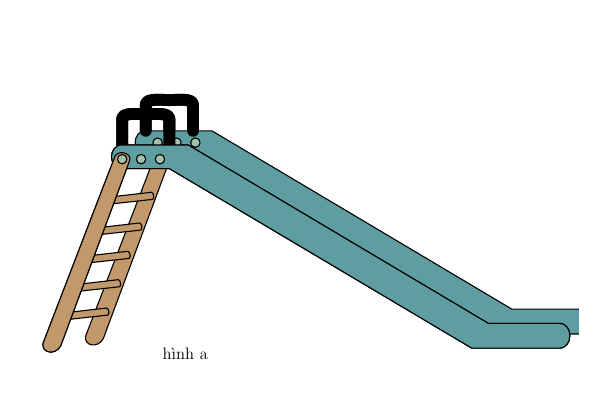
\begin{tikzpicture}[line join=round, line cap=round,scale=0.5,transform shape]
\clip (-6,-5) rectangle (8,4);
\tikzset{cau_truot_1/.pic={
%====================Dài
\draw[line width=1.5mm,shift={(1,.6)}] (-6,1.7)--(-6,2.8)
..controls +(90:.3) and +(180:.3) ..(-5,3)
..controls +(0:.3) and +(90:.3) ..(-4,2.8)--(-4,1.7)
;
\draw[line width=1.5mm] (-6,1.7)--(-6,2.8)
..controls +(90:.3) and +(180:.3) ..(-5,3)
..controls +(0:.3) and +(90:.3) ..(-4,2.8)--(-4,1.7)
;
\def\D{
(-6,1.7)
..controls +(-180:.6) and +(180:.6) ..(-6,.7)--(-4,.7)--(8.8,-6.9)--(12.5,-6.9)..controls +(0:.6) and +(-0:.6) ..(12.5,-5.85)--(9.5,-5.85)--(-3.2,1.7)--cycle
;
}
\fill[shift={(1,.6)},cadetblue] \D;
\draw[shift={(1,.6)},black]\D;
%\fill[cadetblue] \D;
\draw[black]\D;

\draw[fill=cambridgeblue] (-3.7,1.8) circle (.2);
\draw[fill=cambridgeblue] (-2.9,1.8) circle (.2);
\draw[fill=cambridgeblue] (-4.5,1.8) circle (.2);


}}
\tikzset{cau_truot_2/.pic={
\def\T{
(-6.35,1.1)
..controls +(80:.5) and +(60:.4) ..(-5.7,1)--(-8.6,-6.8)
..controls +(-120:.5) and +(-100:.4) ..(-9.35,-6.7)--cycle
;
}

%--------------------------
\def\Th{
(-4.75,-.3)
..controls +(-30:.1) and +(50:.1) ..(-4.7,-.6)--(-6.5,-.8)
..controls +(150:.1) and +(-150:.1) ..(-6.5,-.5)--cycle
;
}

\fill[shift={(1.8,.3)},camel] \T;
\draw[shift={(1.8,.3)},black]\T;

\fill[camel] \Th;
\draw[black]\Th;
\fill[shift={(-.5,-1.3)},camel]\Th;
\fill[shift={(-1,-2.5)},camel]\Th;
\fill[shift={(-1.4,-3.7)},camel]\Th;
\fill[shift={(-1.9,-4.9)},camel]\Th;

\draw[shift={(-.5,-1.3)},black]\Th;
\draw[shift={(-1,-2.5)},black]\Th;
\draw[shift={(-1.4,-3.7)},black]\Th;
\draw[shift={(-1.9,-4.9)},black]\Th;

\fill[camel] \T;
\draw[black]\T;
%====================Dài
\draw[line width=1.5mm,shift={(1,.6)}] (-6,1.7)--(-6,2.8)
..controls +(90:.3) and +(180:.3) ..(-5,3)
..controls +(0:.3) and +(90:.3) ..(-4,2.8)--(-4,1.7)
;
\draw[line width=1.5mm] (-6,1.7)--(-6,2.8)
..controls +(90:.3) and +(180:.3) ..(-5,3)
..controls +(0:.3) and +(90:.3) ..(-4,2.8)--(-4,1.7)
;
\def\D{
(-6,1.7)
..controls +(-180:.6) and +(180:.6) ..(-6,.7)--(-4,.7)--(8.8,-6.9)--(12.5,-6.9)..controls +(0:.6) and +(-0:.6) ..(12.5,-5.85)--(9.5,-5.85)--(-3.2,1.7)--cycle
;
}

\fill[cadetblue] \D;
\draw[black]\D;

\fill[camel] \T;
\draw[black]\T;
\draw[fill=cambridgeblue] (-6,1.1) circle (.2);
\draw[fill=cambridgeblue] (-5.2,1.1) circle (.2);
\draw[fill=cambridgeblue] (-4.4,1.1) circle (.2);


}}

\path
(0,0)pic[scale=0.6]{cau_truot_1}
(0,0)pic[scale=0.6]{cau_truot_2}
;
\draw(-2,-4)node[below]{\large\text{hình a}}
%		(15,-.5)node[below]{\text{hình b}}
%		(15,0)node[below]{$y$ cm}
%		(13,.5)node[left]{$x$ cm}
%		(18,.5)node[right]{$x$ cm}
;
%		\draw(13,1)--(13,0)--(18,0)--(18,1);
%		\draw[dashed](13,1)--(18,1);

\end{tikzpicture}
\begin{tikzpicture}[>=stealth,line join=round,line cap=round,font=\footnotesize,scale=1]
\draw%(-3,-5)node[below]{\text{hình a}}
(3.5,-.5)node[below]{\text{hình b}}
(3.5,0)node[below]{$y$ cm}
(1,.5)node[left]{$x$ cm}
(6,.5)node[right]{$x$ cm}
;
\draw(1,1)--(1,0)--(6,0)--(6,1);
\draw[dashed](1,1)--(6,1);
\end{tikzpicture}\\
Với $x$ đạt giá trị bằng bao nhiêu cm thì cầu trượt đảm bảo an toàn nhất cho trẻ em?
\shortans{$20$}
\loigiai{
Do tấm kim loại có bề rộng 80 cm nên ta có $2x+y=80\Leftrightarrow y=80-2x$.\\
Để có thể thiết kế được máng trượt thì $y>0\Leftrightarrow 80-2x>0\Leftrightarrow x<40$, suy ra $0<x<40$.\\
Diện tích của mặt cắt máng trượt là $S=xy=x\left(80-2x\right)=-2x^2+80x$.\\
Xét $S(x)=-2x^2+80x$ với $x\in\left(0;40\right)$.\\
$S'(x)=-4x+80$;
$S'(x)=0\Leftrightarrow-4x+80=0\Leftrightarrow x=20$.\\
Bảng biến thiên của hàm số $S(x)$ như sau
\begin{center}

\begin{tikzpicture}
\tkzTabInit[nocadre=false,lgt=1.2,espcl=2.5,deltacl=0.6]
{$x$ /0.6,$S'(x)$ /0.6,$S(x)$ /1.7}
{$0$,$20$,$40$}
\tkzTabLine{,+,$0$,-,}
\tkzTabVar{-/$0$, +/$800$,-/$0$}
\end{tikzpicture}
\end{center}
Do đó, hàm số $S(x)$ đạt cực đại tại $x=20$ và $S_C=800$.\\
Vậy để cầu trượt đảm bảo an toàn nhất cho trẻ em thì $x=20$ cm.}
\end{ex}

\begin{ex}%[2D4H3-1]
	\immini[thm]{Cho $(H)$ là hình phẳng được tô đậm trong hình vẽ và được giới hạn bởi các đường có phương trình $y=\dfrac{10}{3}x-x^2$ và $y=\heva{&-x&&\text{ khi }x\le 1\\&x-2&&\text{ khi }x>1}$. Diện tích của $(H)$ bằng bao nhiêu?
	\shortans[]{6,5}
	}{
		\begin{tikzpicture}[scale=.75,>=stealth,font=\footnotesize]
			\draw[->] (-1.5, 0) -- (3.5, 0) node[below] {$x$};
			\draw[->] (0, -1.5) -- (0, 3) node[left] {$y$};
			\draw (0, 0) node[below left] {$O$};
			\draw[domain=0:3,smooth] plot (\x,{10/3*\x - \x*\x});
			\draw[domain=-1:1] plot (\x,{-\x});
			\draw[domain=1:3.5] plot (\x,{\x-2});
			\fill[pattern=north east lines,pattern color=gray!80]
			(0, 0) -- plot[domain=0:1] (\x,{10/3*\x - \x*\x}) -- (1, 2.33) -- (1, -1) -- plot[domain=1:0] (\x,{-\x}) -- cycle;
			\fill[pattern=north east lines,pattern color=gray!80]
			(1, -1) -- (1, 2.33) -- plot[domain=1:3] (\x,{10/3*\x - \x*\x}) -- (3, 1) -- plot[domain=3:1] (\x,{\x-2}) -- cycle;
			\draw[dashed] (1, 0) node[fill=white,above right] {$1$} -- (1, -1) -- (0, -1) node[left] {$-1$};
			\draw[dashed] (3, 0) node[below] {$3$} -- (3, 1);
			\draw[dashed] (2, 0) node[below right] {$2$};
			\fill (1, -1) circle (1pt) node[below right] {$A$};
			\fill (3, 1) circle (1pt) node[ right] {$B$};
			\fill (0, 0) circle (1pt);
			\fill (0, -1) circle (1pt);
			\fill (1, 0) circle (1pt);
			\fill (2, 0) circle (1pt);
			\fill (3, 0) circle (1pt);
		\end{tikzpicture}
	}
	\loigiai{
		Phương trình hoành độ giao điểm của hai đồ thị hàm số $y=-x$ và $y=x-2$ là $-x=x-2\Leftrightarrow x=1$. \\
		Diện tích hình phẳng cần tính là
		\[\begin{aligned}S&=\displaystyle\int \limits_0^1\left[\left(\frac{10}{3}x-x^2\right)-(-x)\right]\mathrm{\,d}x+\displaystyle\int \limits_1^3\left[\left(\frac{10}{3}x-x^2\right)-(x-2)\right]\mathrm{\,d}x\\&=\displaystyle\int \limits_0^1\left(\frac{13}{3}x-x^2\right)\mathrm{\,d}x+\displaystyle\int \limits_1^3\left(\frac{7}{3}x-x^2+2\right)\mathrm{\,d}x\\&=\left(\frac{13}{6}x^2-\frac{x^3}{3}\right)\Bigg|_0^1+\left(\frac{7}{6}x^2-\frac{x^3}{3}+2x\right)\Bigg|_1^3\\&=\left(\frac{13}{6}-\frac{1}{3}\right)+\left[\left(\frac{63}{6}-9+6\right)-\left(\frac{7}{6}-\frac{1}{3}+2\right)\right]\\&=\frac{11}{6}+\left[\frac{15}{2}-\frac{17}{6}\right]=\frac{11}{6}+\frac{14}{3}=\frac{39}{6}=\frac{13}{2}=6{,}5.\end{aligned}\]
		Vậy $S=6{,}5$.
	}
\end{ex}

\begin{ex}%[2D6H1-2]
	Trong một xưởng sản xuất có $800$ bóng đèn, qua kiểm nghiệm chất lượng người ta thấy trong đó có $750$ bóng đèn tốt và $50$ bóng đèn kém không đạt chất lượng. Các bóng đèn tốt có $3$ màu: đỏ, trắng, xanh và số bóng đèn màu đỏ chiếm $40\%$. Chọn ra ngẫu nhiên một bóng trong $800$ bóng đèn. Xác suất để bóng đèn được chọn có màu đỏ, biết rằng bóng đèn đó tốt là bao nhiêu?
	\shortans[]{0,4}
	\loigiai{
		Xét các biến cố: \\
		$A$: \lq\lq Bóng được chọn có màu đỏ\rq\rq.\\
		$B$: \lq\lq Bóng được chọn là bóng tốt\rq\rq.\\
		Số bóng đèn tốt là $n(B)=750$ (bóng).\\
		Số bóng đèn tốt có màu đỏ là $n(A\cap B)=750\cdot 40\%=300$ (bóng). \\
		Xác suất để bóng đèn được chọn có màu đỏ, biết rằng bóng đèn đó tốt là
		\[\mathrm{P}(A\mid B)=\dfrac{n(A\cap B)}{n(B)}=\dfrac{300}{750}=\dfrac{2}{5}=0{,}4.\]
	}
\end{ex}

\begin{ex}%[2D1H3-6]
	Ông A định đúc một hố ga bằng bê tông dạng hình hộp chữ nhật có đáy là hình vuông và có thể tích bằng $4$ m$^3$. Hỏi diện tích đáy hố ga bằng bao nhiêu mét vuông để khi đúc ông A tiết kiệm nguyên liệu nhất?
	\shortans[]{4}
	\loigiai{
		Gọi $a$ và $b$ lần lượt là chiều dài cạnh đáy và chiều cao hố ga ($a$, $b>0$). \\
		Thể tích hố ga là $V=a^2b=4\Rightarrow b=\dfrac{4}{a^2}$. \\
		Diện tích toàn phần (không tính nắp) hố ga là $S=a^2+4ab=a^2+4a\left(\dfrac{4}{a^2}\right)=a^2+\dfrac{16}{a}$. \\
		Để tiết kiệm nguyên liệu nhất thì diện tích toàn phần phải nhỏ nhất. Ta có thể giải quyết bằng các cách sau
		\begin{itemize}
			\item \textbf{Cách 1: Sử dụng bất đẳng thức AM-GM}\\
			Áp dụng bất đẳng thức AM-GM (Cauchy) cho $3$ số dương, ta có
			\[S=a^2+\frac{8}{a}+\frac{8}{a}\ge 3\sqrt[3]{a^2\cdot \frac{8}{a}\cdot \frac{8}{a}}=3\sqrt[3]{64}=12.\]
			Dấu \lq\lq =\rq\rq\ xảy ra khi $a^2=\dfrac{8}{a}\Leftrightarrow a^3=8\Leftrightarrow a=2$. 			
			\item \textbf{Cách 2: Sử dụng đạo hàm}\\
			Xét hàm số $S(a)=a^2+\dfrac{16}{a}$ với $a>0$.\\
			Ta có $S'(a)=2a-\dfrac{16}{a^2}=\dfrac{2a^3-16}{a^2}$.\\
			$S'(a)=0\Leftrightarrow 2a^3-16=0\Leftrightarrow a^3=8\Leftrightarrow a=2$.\\
			Bảng biến thiên
			\begin{center}
				
\begin{tikzpicture}
					\tkzTabInit[nocadre=false,lgt=1.5,espcl=3]
					{$a$ / 1, $S'(a)$ / 1, $S(a)$ / 2}
					{$0$, $2$, $+\infty$}
					\tkzTabLine{ d, -, 0, +, }
					\tkzTabVar{ D+/ $+\infty$, -/ $12$, +/ $+\infty$ }
				\end{tikzpicture}
			\end{center}
		\end{itemize}
		Dựa vào bảng biến thiên, hàm số $S(a)$ đạt giá trị nhỏ nhất tại $a=2$.\\
		Khi đó diện tích đáy hố ga là $S_{\text{ đáy}}=a^2=2^2=4$ (m$^2$).
	}
\end{ex}

\begin{ex}%[2D1H2-1]
	Đường thẳng $\Delta$ có phương trình $y=2x+1$ cắt đồ thị của hàm số $y=x^3-x+3$ tại hai điểm $A$ và $B$ với tọa độ được kí hiệu lần lượt là $A(x_A;y_A)$ và $B(x_B;y_B)$ trong đó $x_B<x_A$. Tìm $x_B+y_B$.
	\shortans[]{-5}
	\loigiai{
		Phương trình hoành độ giao điểm
		\[\begin{aligned}&x^3-x+3=2x+1\\\Leftrightarrow \;&x^3-3x+2=0\\\Leftrightarrow \;&(x-1)^2(x+2)=0\\\Leftrightarrow \;&\hoac{&x=1\\&x=-2.}\end{aligned}\]
		Đường thẳng $\Delta$ cắt đồ thị tại hai điểm phân biệt có hoành độ giao điểm là $x=1$ và $x=-2$. \\
		Theo giả thiết $x_B<x_A$ nên $x_B=-2$ và $x_A=1$. \\
		Thay $x_B=-2$ vào phương trình $y=2x+1$, ta được $y_B=2\cdot (-2)+1=-3$. \\
		Vậy $x_B+y_B=-2+(-3)=-5$.
	}
\end{ex}

\Closesolutionfile{ans}
\indapan{4}{ans/De-TB-Yeu-So-3}
